\documentclass{article}
\usepackage{graphicx}
\usepackage{placeins}
\usepackage[margin=1in]{geometry}


\begin{document}
\begin{titlepage}
   \vspace*{\stretch{1.0}}
   \begin{center}
      \Large\textbf{Supplemental Figures}\\
      \vspace{1em}
      \Large{Chemotherapy weakly contributes to predicted neoantigen expression in ovarian cancer} \\
      \vspace{1em}
     \large\textit{Timothy O'Donnell, Elizabeth L. Christie, Arun Ahuja, Jacqueline Buros, B. Arman Aksoy, David D. L. Bowtell, Alexandra Snyder, Jeff Hammerbacher}
    % \large\textit{O’Donnell et al.}
   \end{center}
   \vspace*{\stretch{2.0}}
\end{titlepage}

% See http://tex.stackexchange.com/questions/168169/options-for-supplementary-materials-in-preprint-version-revtex-arxiv
\setcounter{equation}{0}
\setcounter{figure}{0}
\setcounter{table}{0}
\makeatletter
\renewcommand{\theequation}{S\arabic{equation}}
\renewcommand{\thefigure}{S\arabic{figure}}

\begin{figure}
\centering
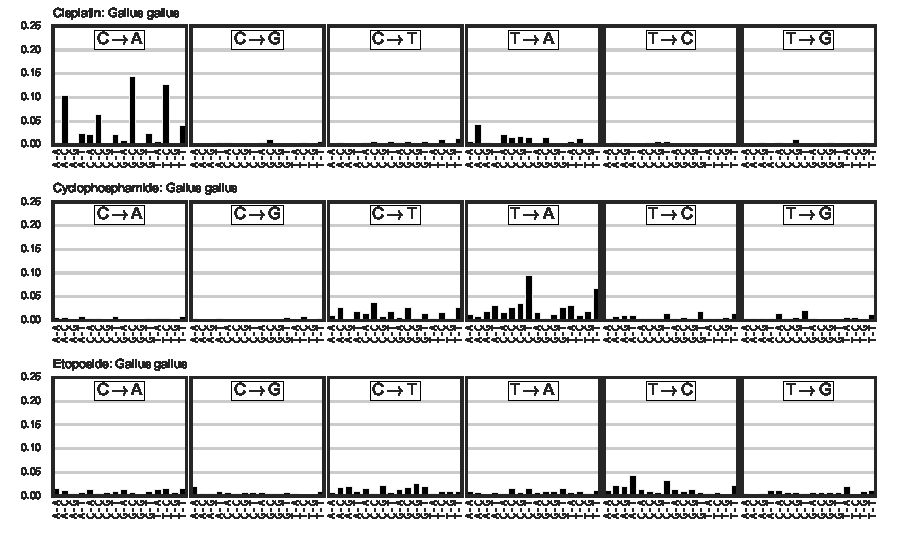
\includegraphics[scale=1.0]{../figures/extracted_signatures_chicken.pdf}
\caption{\textbf{Mutational signatures extracted from Szikriszt et al.}~\cite{Szikriszt_2016}}
\label{fig:supp_extracted_signatures_chicken}
\end{figure}

\begin{figure}
\centering
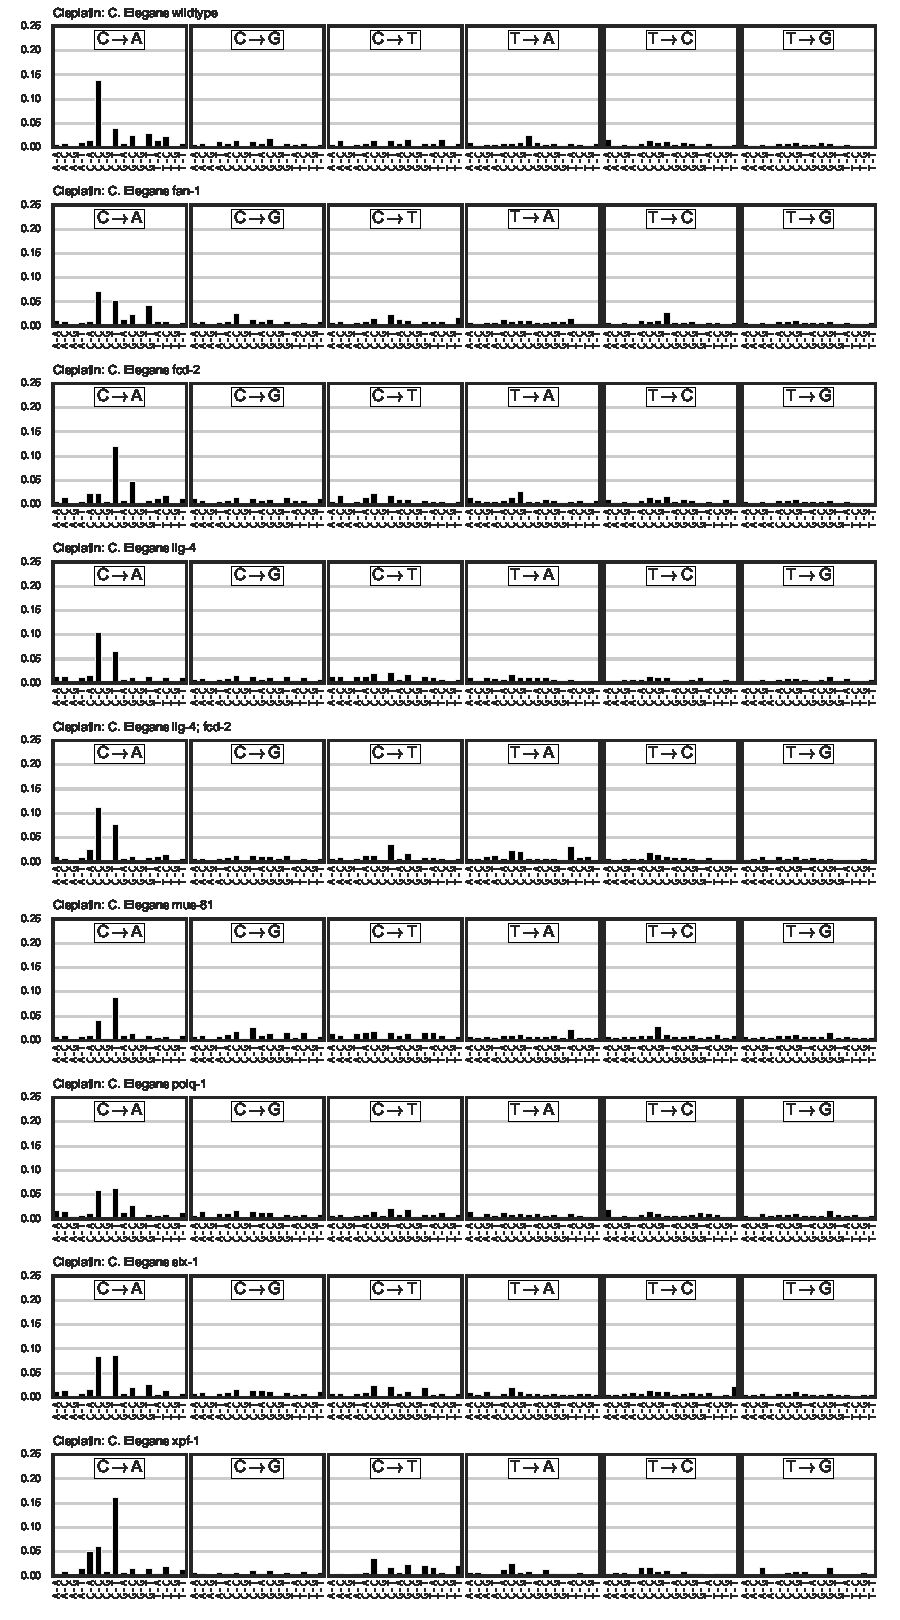
\includegraphics[scale=1.0]{../figures/extracted_signatures_worm.pdf}
\caption{\textbf{Mutational signature extracted from Meier et al.}~\cite{Meier_2014}}
\label{fig:supp_extracted_signatures_worm}
\end{figure}

\begin{figure}
\centering
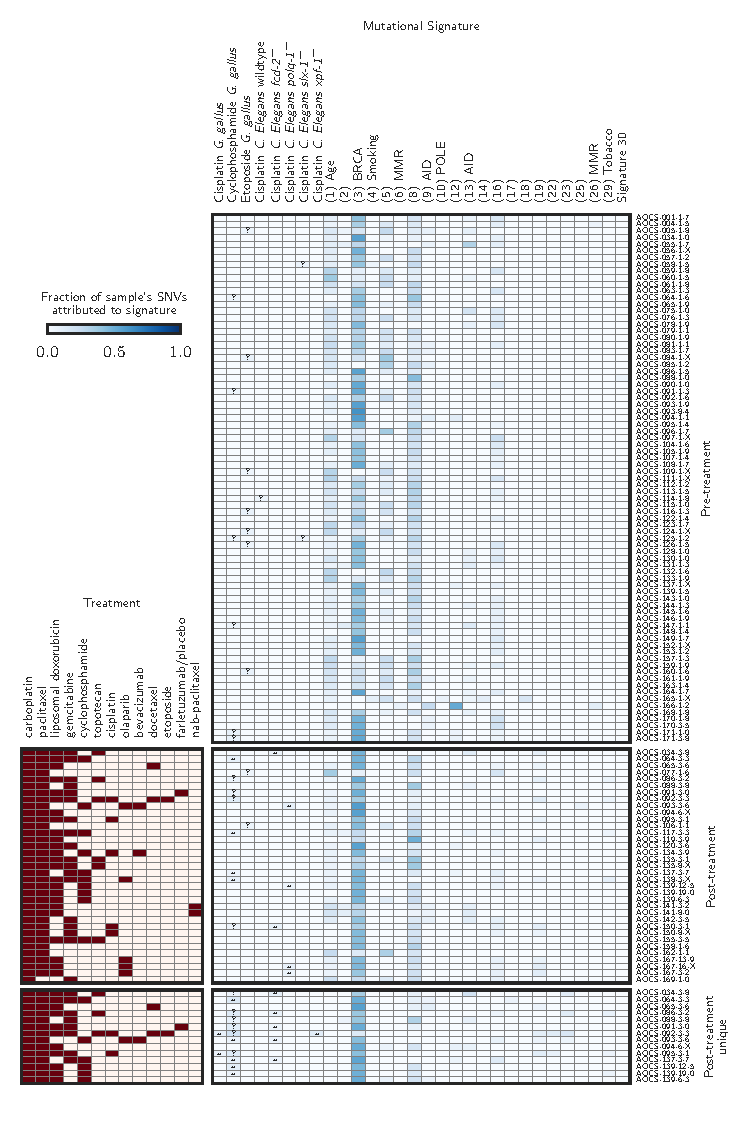
\includegraphics[scale=1.0]{../figures/supplementary_signatures.pdf}
\caption{\textbf{Detected mutational signatures across all samples.} The symbols are as in main text Figure~1. The top and middle panels show the signature deconvolutions for all pre- and post-treatment samples, respectively. The bottom panel shows deconvolutions for the mutations unique to the paired post-treatment samples, requiring high coverage and no variant reads in the donor-matched pre-treatment sample.}
\label{fig:supp_signatures}
\end{figure}

\begin{figure}
\centering
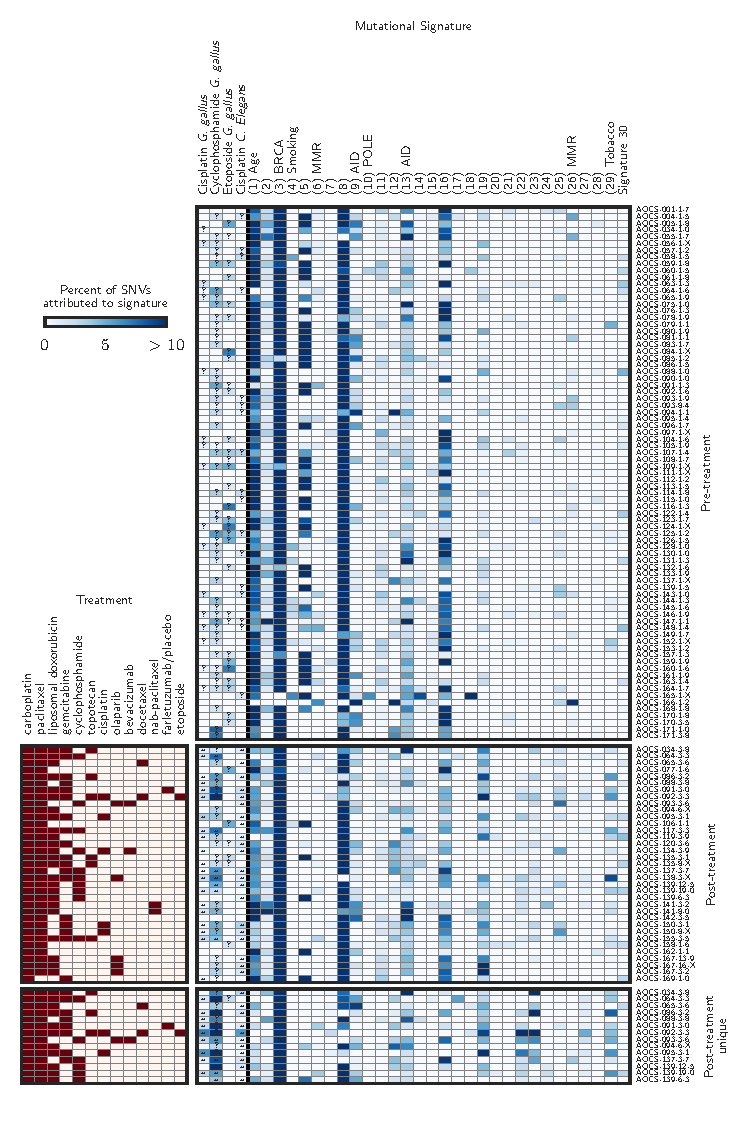
\includegraphics[scale=1.0]{../figures/supplementary_signatures_no_cutoff.pdf}
\caption{\textbf{Mutational signature deconvolutions without any threshold of detection.} Here, signatures accounting for less than the 6\% recommended detection threshold are included.}
\label{fig:supplementary_signatures_no_cutoff}
\end{figure}

\begin{figure}
\centering
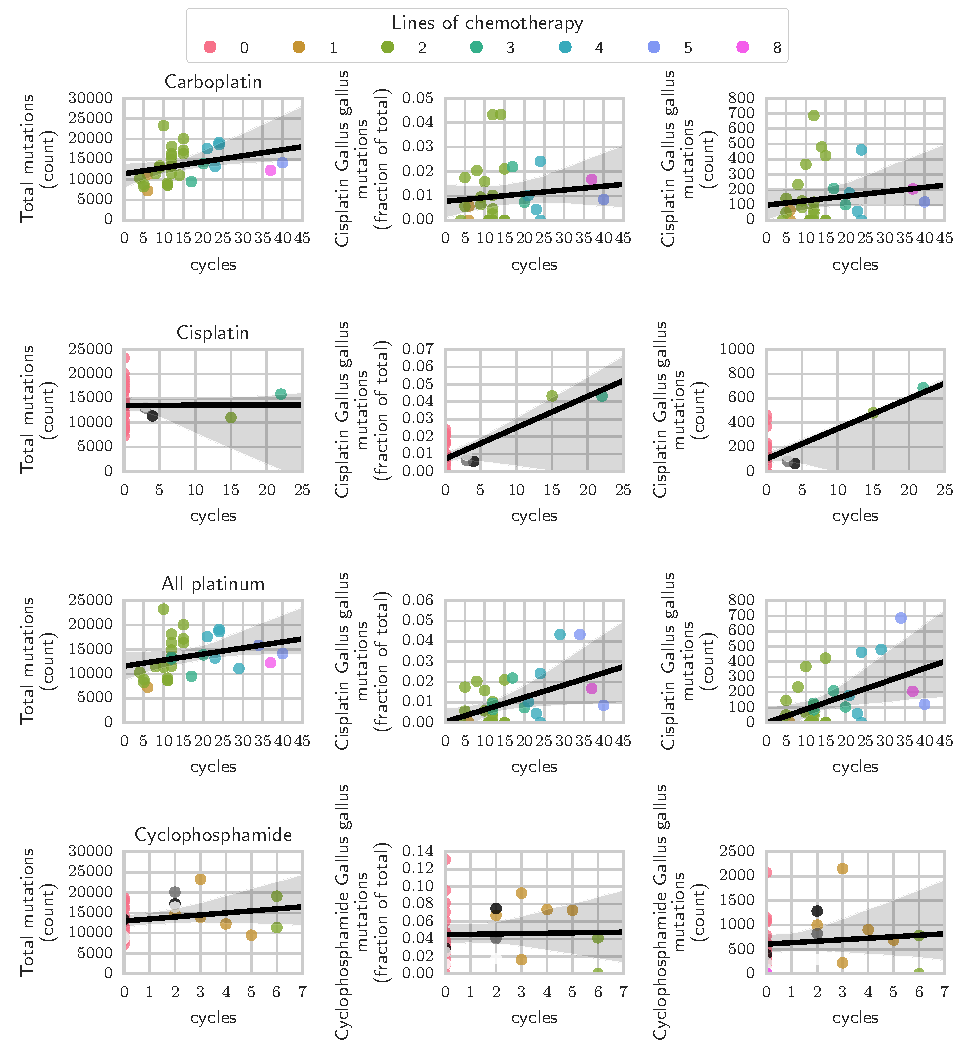
\includegraphics[scale=1.0]{../figures/chemo_cycles_and_mutations.pdf}
\caption{\textbf{Association of chemotherapy cycles on total genome-wide mutation burden (left) and mutations attributed to the \textit{G. Gallus} cisplatin and cyclophosphamide signatures as a fraction of total (middle) and as a count (right)}. The total mutation burden includes both SNVs and indels. Cycles indicated are of the labelled chemotherapy. Colors indicate the number of lines of chemotherapy.}
\label{fig:supp_chemo_cycles_and_mutations}
\end{figure}

\begin{figure}
\centering
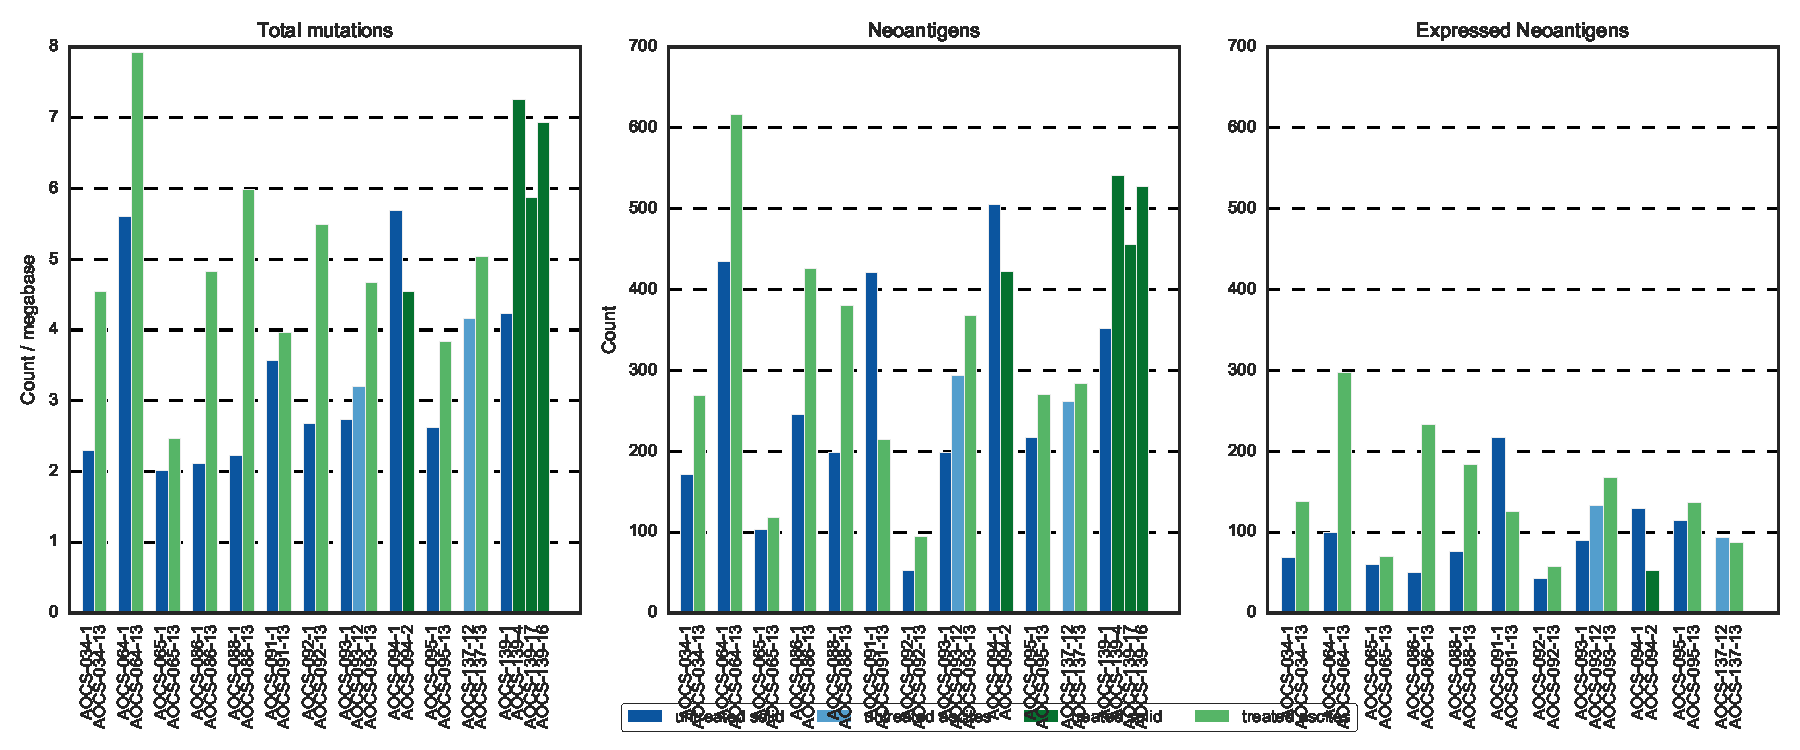
\includegraphics[scale=1.0]{../figures/paired_counts.pdf}
\caption{\textbf{Mutations, neoantigens, and expressed neoantigens for donor-matched primary/untreated and relapse/treated samples.}}
\label{fig:supp_paired}
\end{figure}

\begin{figure}[htbp]
\centering
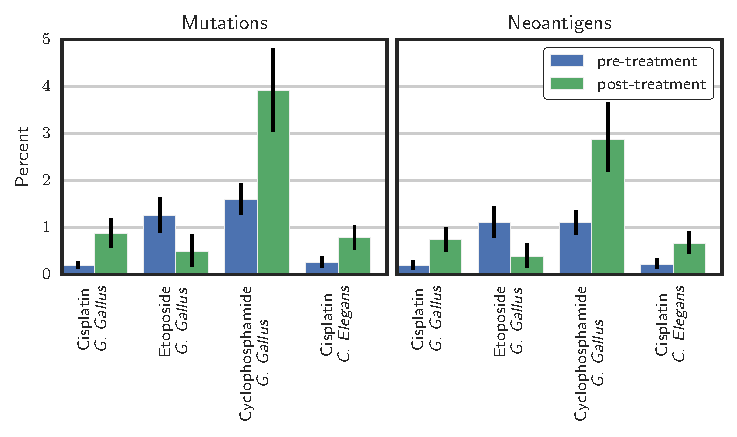
\includegraphics[scale=1.0]{../figures/sources_of_mutations_and_neoantigens_ungrouped.pdf}
\caption{\textbf{Contribution of chemotherapy SNV signatures.} The fraction of each sample's mutations, neoantigens, and expressed neoantigens attributed to putative chemotherapy signatures is shown. Bars give the mean, and points indicate individual samples.}
\label{fig:sourcesungrouped}
\end{figure}

\begin{figure}[htbp]
\centering
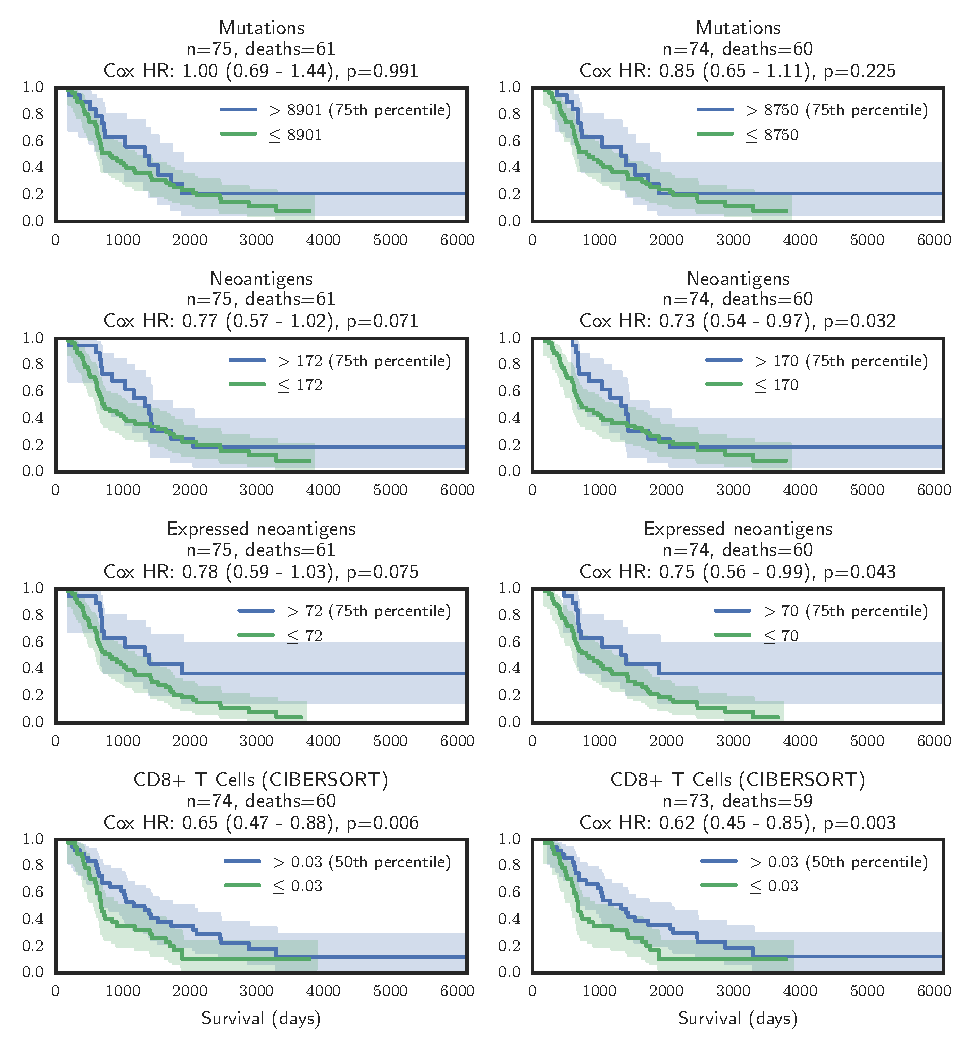
\includegraphics[scale=1.0]{../figures/survival.pdf}
\caption{\textbf{Kaplan-Meier curves for patients split by the number of mutations, neoantigens, expressed neoantigens, or estimate of CD8+ T cell infiltrate.} Only primary/untreated solid-tissue samples are considered. The survival curves split the samples into high and low groups using a percentile threshold, but the annotated Cox hazard ratio (HR) and p-value correspond to a regression model that treats the value of interest as a continuous covariate. The left plots include all primary/untreated samples; the right plots exclude outlier sample AOCS-166-1-2. The CD8+ T cell analyses exclude sample AOCS-056-1-X, which failed deconvolution.}
\label{fig:survival}
\end{figure}

\begin{figure}[htbp]
\centering
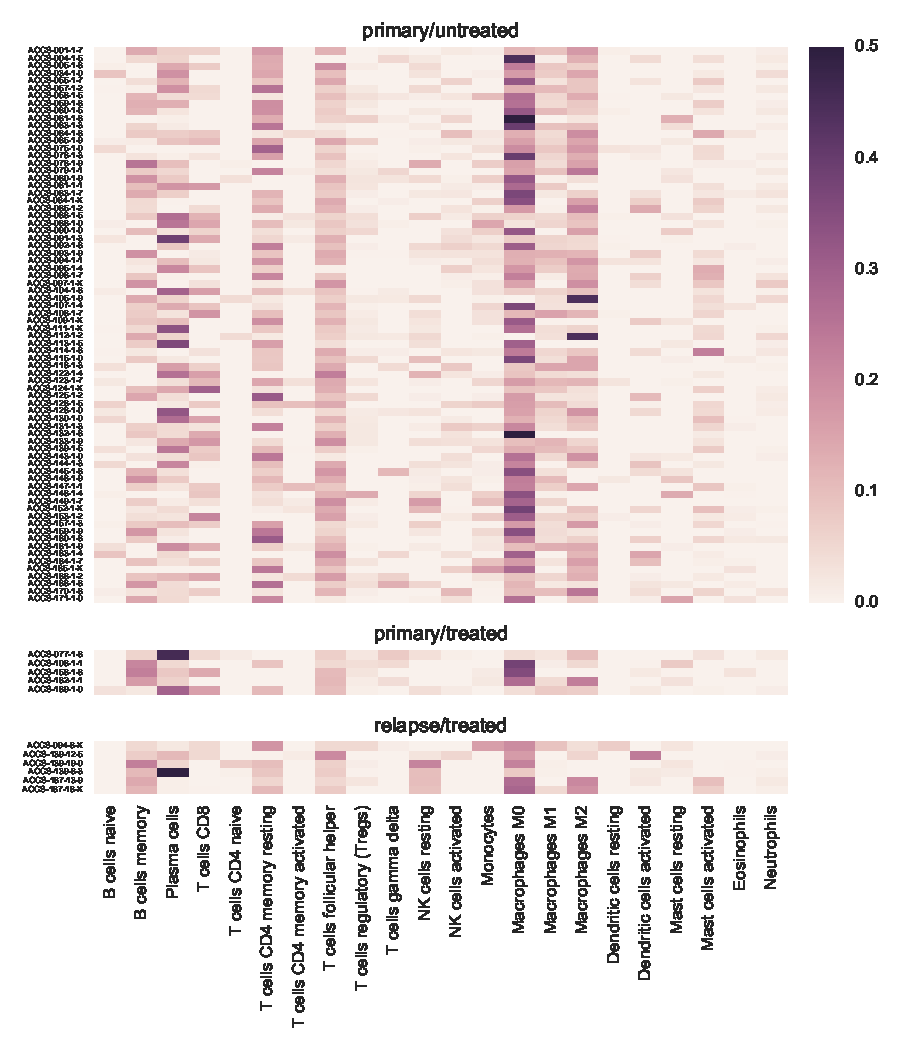
\includegraphics[scale=1.0]{../figures/cibersort_heatmap_solid.pdf}
\caption{\textbf{RNA-seq based immune deconvolution (CIBERSORT) of solid-tissue samples.}}
\label{fig:cibersortsolid}
\end{figure}

\begin{figure}[htbp]
\centering
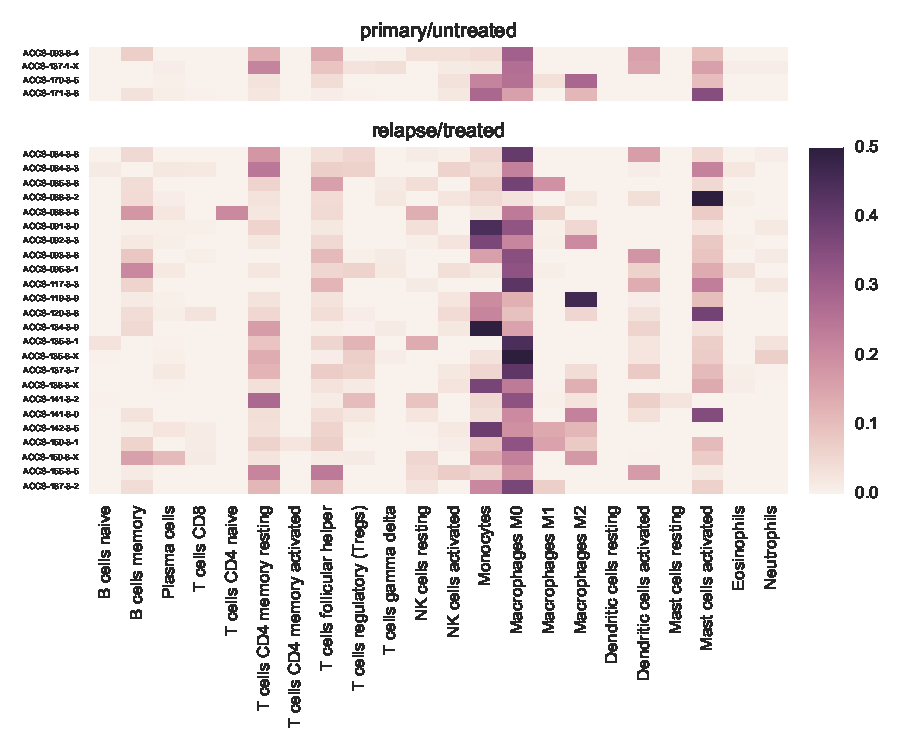
\includegraphics[scale=1.0]{../figures/cibersort_heatmap_ascites.pdf}
\caption{\textbf{RNA-seq based immune deconvolution (CIBERSORT) of ascites samples.}}
\label{fig:cibersortascites}
\end{figure}


\begin{figure}[htbp]
\centering
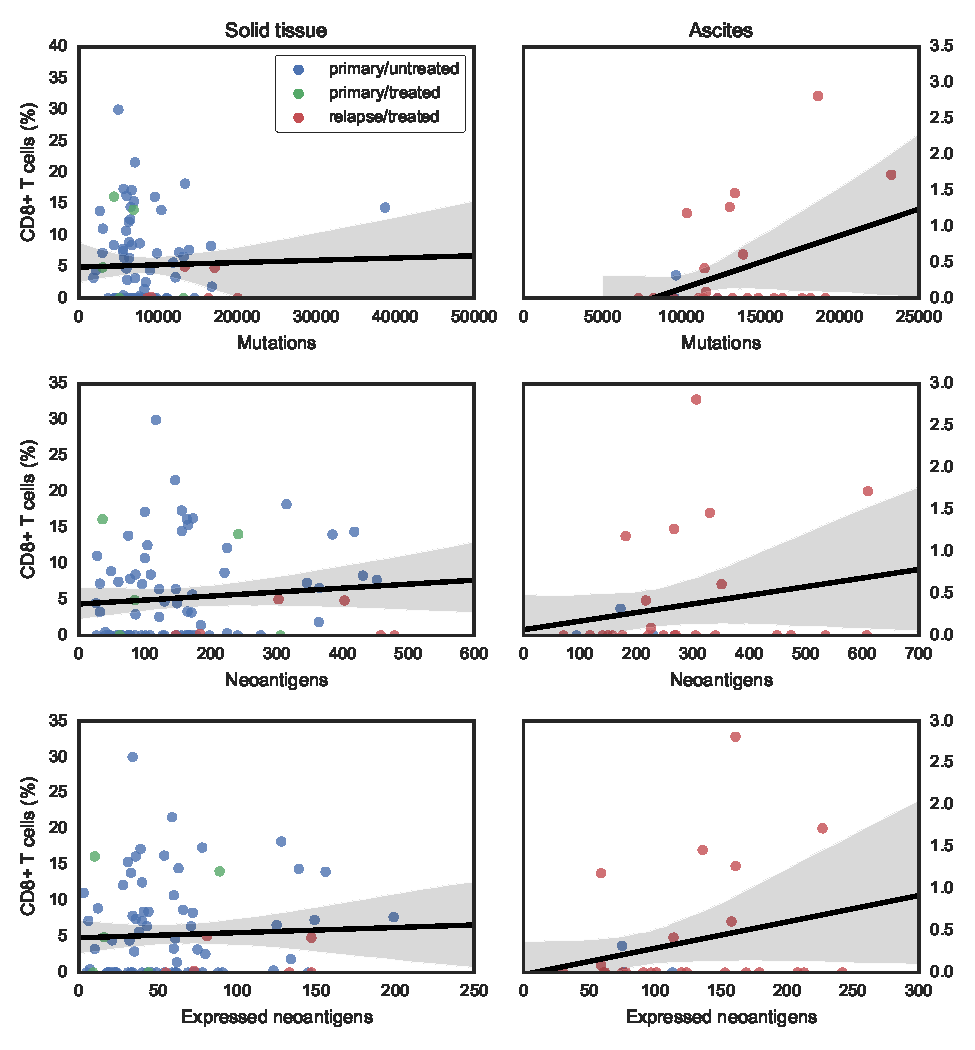
\includegraphics[scale=1.0]{../figures/cd8_vs_muts.pdf}
\caption{\textbf{Relationship between CD8+ T cell infiltrate estimated by CIBERSORT and mutations, neoantigens, or expressed neoantigens for solid tissue (left) and ascites (right) samples.} Colors indicate sample time point.}
\label{fig:cd8vsmuts}
\end{figure}


\newpage
\FloatBarrier

\bibliography{bmc_article} 
\bibliographystyle{ieeetr}

\end{document}